\subsubsection{Overview}
\label{Connor-Stevens Neuron}
\index{Connor-Stevens Neuron}\index{utilities, Connor-Stevens Neuron}
\begin{figure}[h]
\begin{center}
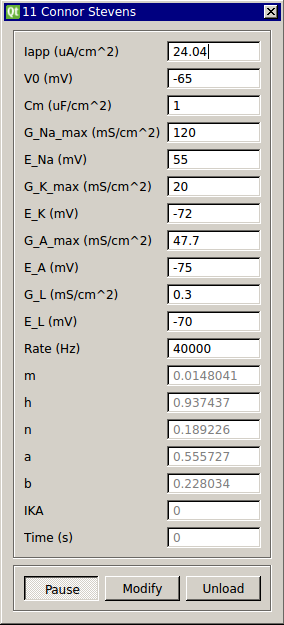
\includegraphics[width=2in]{csneuron.png} 
\caption[CS Neuron]{GUI for a real-time Connor-Stevens neuron within RTXI.} 
\end{center}
\label{csneuron}
\end{figure}

The Connor Stevens model neuron is like the Hodgkin-Huxley neuron, but with slightly different kinetics for the fast sodium and potassium delayed-rectifier channels and an additional A-type potassium channel (Dayan and Abbott, Theoretical Neuroscience, Ch. 6). These changes give the Connor Stevens neuron Type I excitability such that it can achieve arbitrarily low spike rates. This feature may make this model more useful for testing custom modules than the Hodgkin-Huxley model neuron.

\subsubsection{Input Channels}
\begin{description}
\item[input(0)- Iapp] applied current (A)
\end{description}

\subsubsection{Output Channels}
\begin{description}
\item[output(0) - Vm] membrane voltage (V)
\end{description}

\subsubsection{Parameters}
\begin{description}
\item[V0] voltage (mV)
\item[Cm] membrane capacitance (uF/cm\^2)
\item[G\_Na\_max] max. Na+ conductance density  (mS/cm\^2)
\item[E\_Na] Na+ reversal potential (mV)
\item[G\_K\_max] max. K+ conductance density (mS/cm\^2)
\item[E\_K] K+ reversal potential (mV)
\item[G\_A\_max] max. transient A-type K+ conductance density (mS/cm\^2)
\item[E\_A] A-type K+ reversal potential (mV) 
\item[G\_L] leak channel conductance density (mS/cm\^2)
\item[E\_L] leak channel reversal potential (mV)
\item[rate] rate of integration (Hz)
\end{description}

\subsubsection{States}
\begin{description}
\item[m] sodium activation
\item[h] sodium inactivation
\item[n] potassium inactivation
\item[a] A-type potassium activation
\item[b] A-type potassium inactivation
\item[IKA] A-type potassium current
\item[Time] time (s)
\end{description}